\documentclass[paper=a4, fontsize=12pt]{scrartcl} % A4 paper and 11pt font size

\usepackage{euler} % Use the Adobe Utopia font for the document - comment this line to return to the LaTeX default
\usepackage[english]{babel} % English language/hyphenation
\usepackage{amsmath,amsfonts,amsthm} % Math packages
\interdisplaylinepenalty=2500
\usepackage{amssymb}
\usepackage{hyperref}

\newtheorem{thm}{Theorem}[section]
\newtheorem{lem}[thm]{Lemma}
\newtheorem{prop}[thm]{Proposition}
\newtheorem{cor}[thm]{Corollary}
\newtheorem{conj}[thm]{Conjecture}
\theoremstyle{definition}
\newtheorem{defn}[thm]{Definition}
\usepackage{sectsty} % Allows customizing section commands
\allsectionsfont{\centering \normalfont\scshape} % Make all sections centered, the default font and small caps

\usepackage{graphicx,wrapfig,lipsum}
\usepackage{fancyhdr} % Custom headers and footers
\pagestyle{fancyplain} % Makes all pages in the document conform to the custom headers and footers
\fancyhead{} % No page header - if you want one, create it in the same way as the footers below
\fancyfoot[L]{} % Empty left footer
\fancyfoot[C]{} % Empty center footer
\fancyfoot[R]{\thepage} % Page numbering for right footer
\renewcommand{\headrulewidth}{0pt} % Remove header underlines
\renewcommand{\footrulewidth}{0pt} % Remove footer underlines
\setlength{\headheight}{13.6pt} % Customize the height of the header

\numberwithin{equation}{section} % Number equations within sections (i.e. 1.1, 1.2, 2.1, 2.2 instead of 1, 2, 3, 4)
\numberwithin{figure}{section} % Number figures within sections (i.e. 1.1, 1.2, 2.1, 2.2 instead of 1, 2, 3, 4)
\numberwithin{table}{section} % Number tables within sections (i.e. 1.1, 1.2, 2.1, 2.2 instead of 1, 2, 3, 4)

\setlength\parindent{0pt} % Removes all indentation from paragraphs - comment this line for an assignment with lots of text

%----------------------------------------------------------------------------------------
%	TITLE SECTION
%----------------------------------------------------------------------------------------

\newcommand{\horrule}[1]{\rule{\linewidth}{#1}} % Create horizontal rule command with 1 argument of height

\title{	
\normalfont \normalsize
\textsc{Addis Ababa university} \\ [25pt] % Your university, school and/or department name(s)
\horrule{0.5pt} \\[0.4cm] % Thin top horizontal rule
\huge Triangle Inequality \\ % The assignment title
\horrule{2pt} \\[0.5cm] % Thick bottom horizontal rule
}

\author{Miliyon T.} % Your name

\date{\normalsize\today} % Today's date or a custom date

\begin{document}

\maketitle % Print the title


\begin{abstract}
  Abstract: \textbf{Triangle Inequality} is one of the most important inequalities in mathematics.There are four proofs presented here and each of them are proved
  by using different areas of mathematics.
\end{abstract}

\begin{defn}[Triangular inequality]
 The sum of the lengths of any two sides of a triangle is greater than the length of the third side.
\end{defn}
\section{Geometry}
%------------------------------------------
\begin{wrapfigure}{r}{5cm}
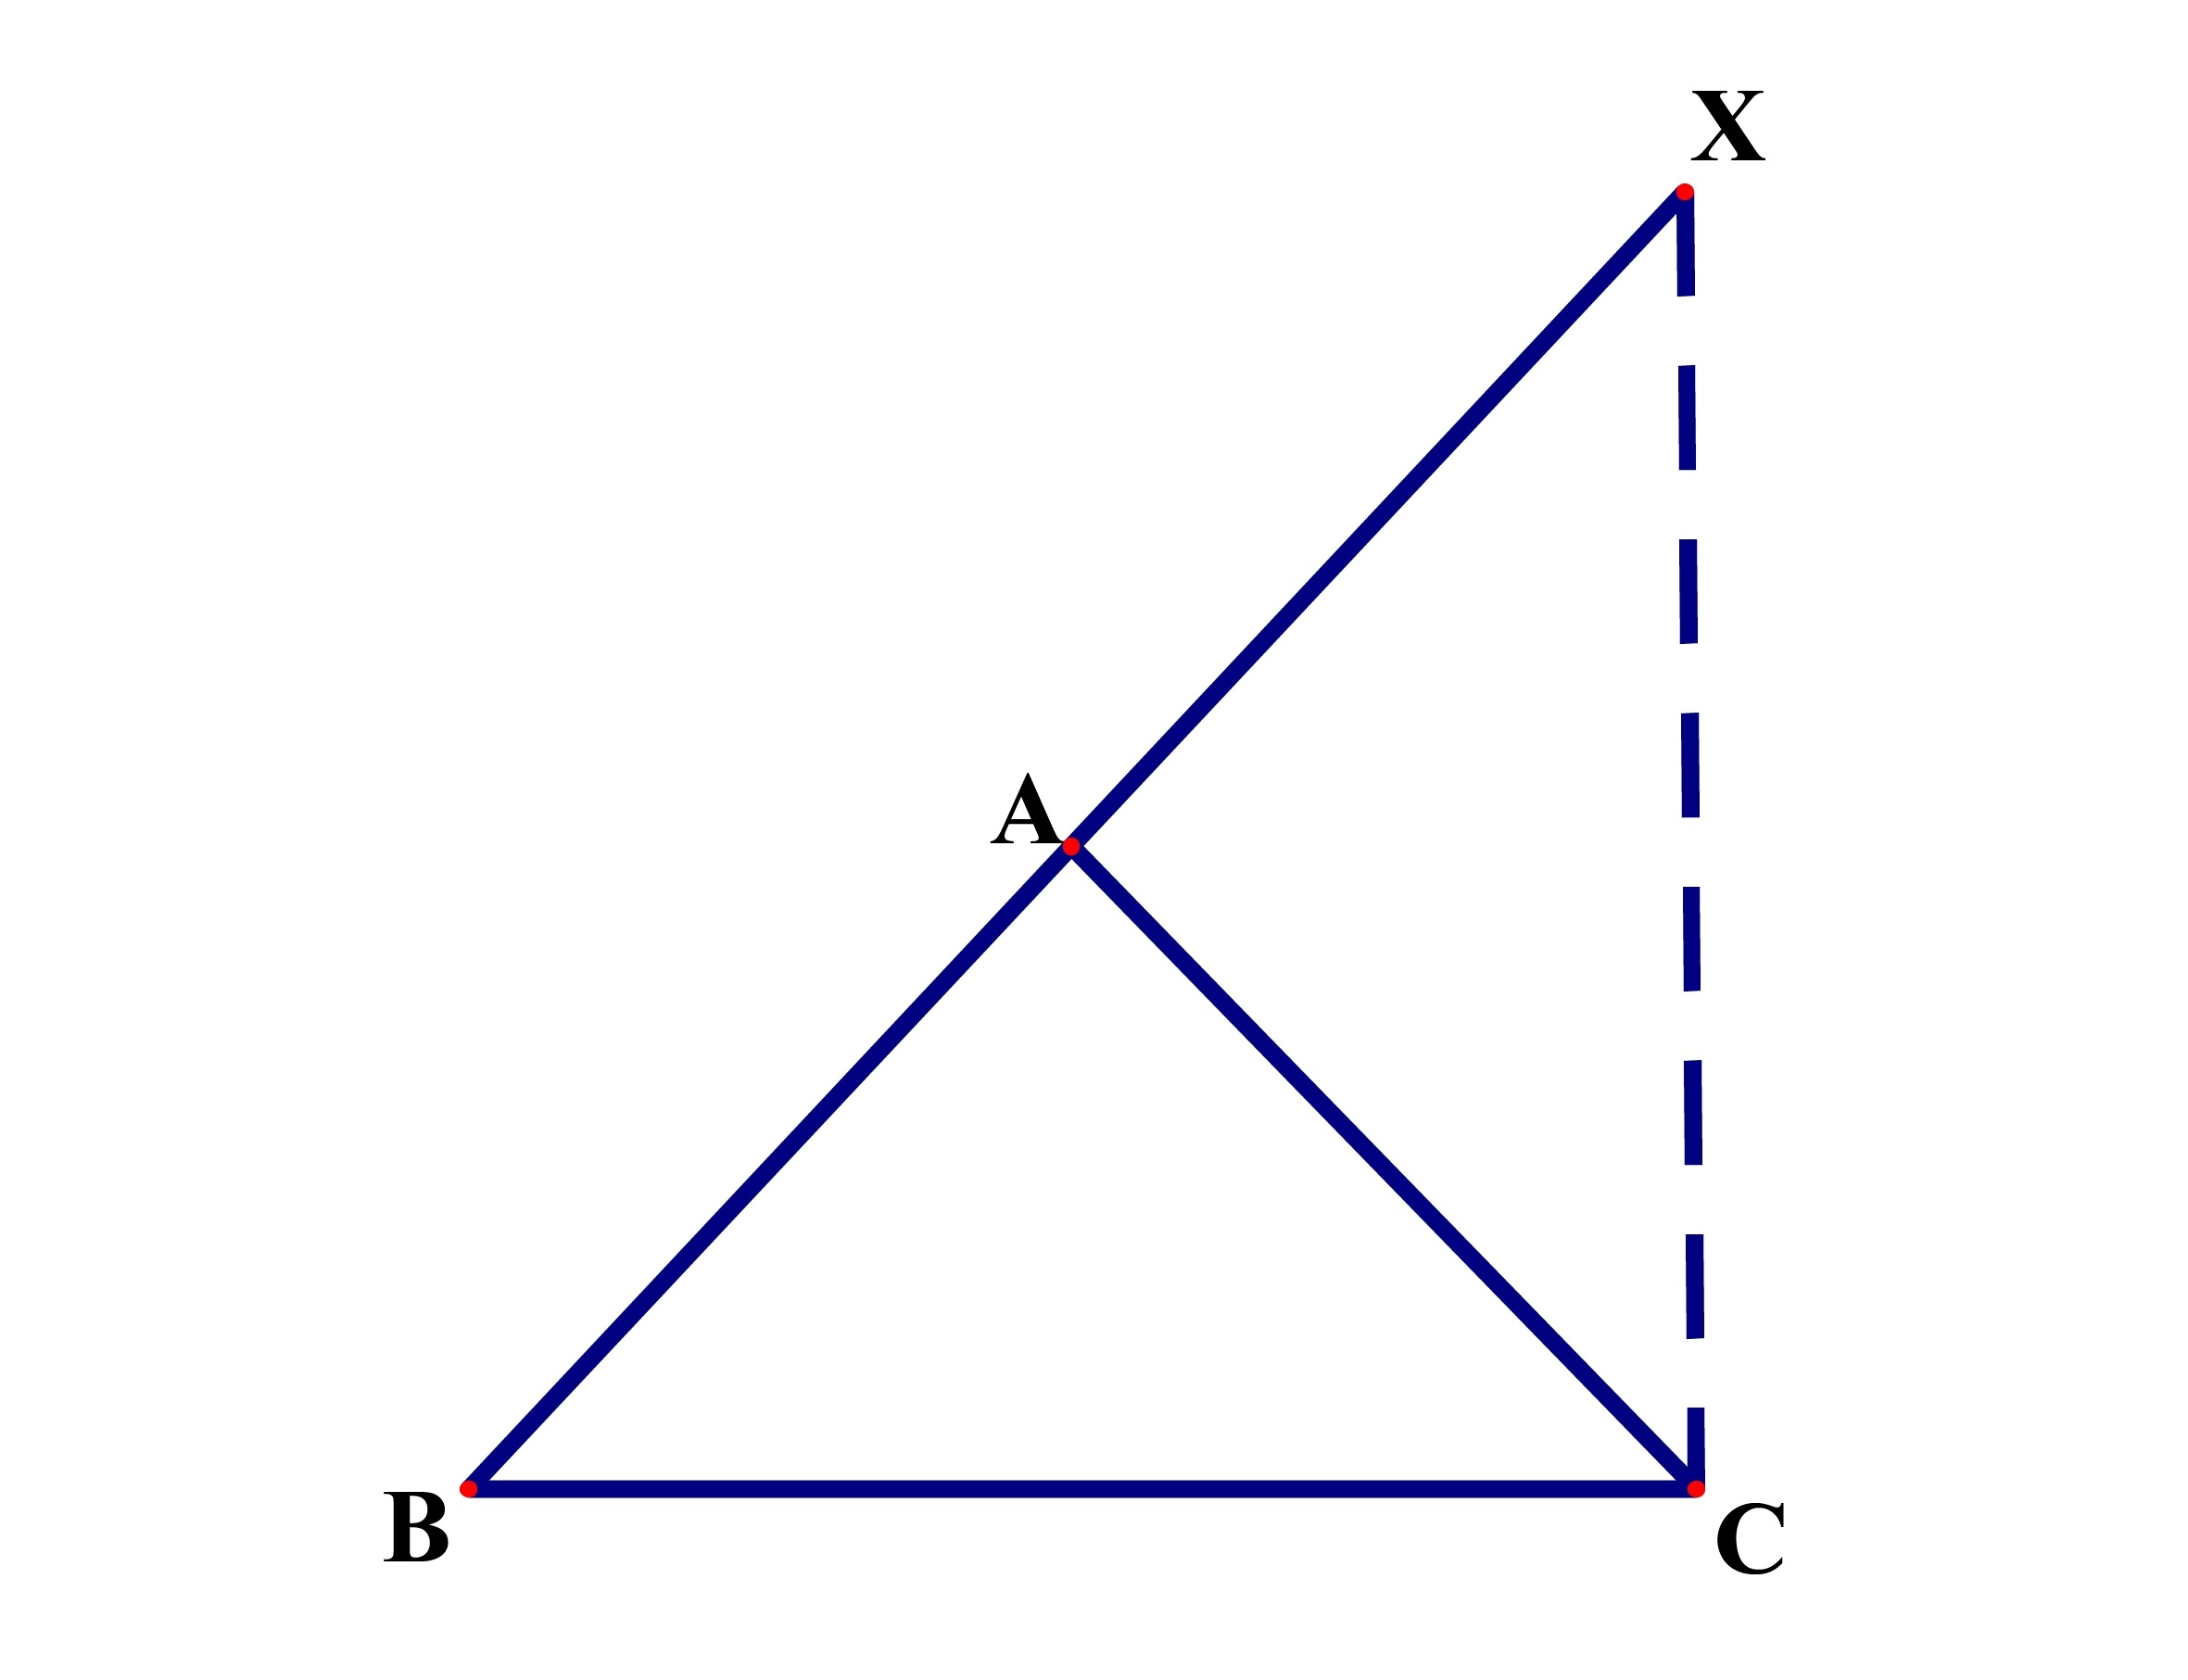
\includegraphics[width=7cm]{7.jpg}
\caption{1234}\label{wrap-fig:1}
\end{wrapfigure}
%------------------------------------------
\textit{Proof}:

Let ABC be a triangle. We need to show that $BA + AC > BC$,
$BA + BC > AC$ and $BC + AC > BA$. \\We show only $BA + AC > BC$. The others can be shown in similar manner. See the Figure on the right

Extend $\overline{BA}$  to some point X on $\overleftrightarrow{AB}$ such that $B-A-X$  and
$\overline{AX} \equiv \overline{AC}$. This is possible by Axiom of segment construction.
Join C and X.  Since $\overline{AX} \equiv \overline{AC}$ and $A\hat{X}C\equiv X\hat{C}A$.  $XCA<XCB$ by definition
of angle comparison.  Thus, $A\hat{X}C<X\hat{C}B$(i.e. $B\hat{X}C<X\hat{C}B$).
Now in $\triangle BCX$ we have $BC < BX$.
But $BX = BA + AX$ (as B, A, X are collinear and $B-A-X$ ,$ BX = BA + AC$  as $\overline{AC}\equiv \overline{AX}$.
Therefore,
\begin{align*}
BC < BA + AC
\end{align*}


\section{Algebra}
\begin{thm}[Triangle inequality] $|x+y|\leq |x|+|y|$

\begin{proof}
From the definition of absolute value we have

$$x\leq |x|\qquad \text{and}\qquad -x\leq |x|$$
$$y\leq |y|\qquad \text{and}\qquad -y\leq |y|$$
\begin{equation}
x+y\leq |x|+|y|
\end{equation}

And
\begin{equation}
 -(x+y)\leq |x|+|y|
\end{equation}
From 2.1 and 2.2 we can conclude that
$$-(|x|+|y| )\leq x+y\leq (|x|+|y|)$$
$$\Rightarrow|x+y|\leq |x|+|y|$$

\end{proof}
\end{thm}
\section{Complex Analysis}
\begin{defn}
 Let $z=x+iy$ be complex number with real part $x$ ($\text{Re}(z)=x$) and imaginary part $y$ ($\text{Im}(z)=y$), then the conjugate of $z$ is defined by $\bar{z}=x-iy$.\\ Norm of $z$ is given by $|z|=\sqrt{x^2+y^2} $.
\end{defn}
\begin{thm}[Triangle inequality]
\begin{align}
|z_1+z_2 |\leq |z_1 |+|z_2 |
\end{align}
\begin{proof}
$$|z_1+z_2 |^2=(z_1+z_2)\overline{(z_1+z_2)}$$

\begin{align*}
  (z_1+z_2)\overline{(z_1+z_2)}  &=z_1 \overline{(z_1+z_2)}+z_2 \overline{(z_1+z_2)}\\
                                 &=z_1 \overline{(z_1)}+z_1 \overline{(z_2)}+z_2 \overline{(z_1)}+z_2 \overline{(z_2)}\\
                                 &=|z_1|^2+\overline{\overline{z_1}z_2}+\overline{z_1\overline{z_2}}+|z_2 |^2 \\
                                 &= |z_1|^2+2\text{Re}(z_1\overline{z_2})+|z_2|^2, \qquad \text{since}\quad \text{Re}(z) =\frac{z+\overline{z}}{2}.\\
                                 &\leq |z_1|^2+2|z_1||z_2|+|z_2|^2
\end{align*}

$$\Rightarrow |z_1+z_2|^2\leq (|z_1|+|z_2|)^2$$
$$\Rightarrow  |z_1+z_2|\leq |z_1 |+|z_2|  $$

\end{proof}
\end{thm}
\section{Vector Analysis}

\begin{lem}[Cauchy-Schwartz inequality]
\begin{align}
\|\vec{A}\cdot \vec{B}\|\leq \|\vec{A}\|\|\vec{B}\|
\end{align}
\begin{proof}
$$|\cos(\theta)|\leq 1$$
$$-|\vec{A}||\vec{B}|\leq |\vec{A}||\vec{B}|\cos(\theta) \leq |\vec{A}||\vec{B}|$$
$$-|\vec{A}||\vec{B}|\leq |\vec{A}\cdot \vec{B}|\leq |\vec{A}||\vec{B}|$$
$$\|\vec{A}\cdot \vec{B}\|\leq \|\vec{A}\|\|\vec{B}\|$$
\end{proof}
\end{lem}
\begin{thm}[Triangular inequality]
\begin{align}
\|\vec{A}+ \vec{B}\|\leq \|\vec{A}\|+\|\vec{B}\|
\end{align}
\begin{proof}
$$\|\vec{A}+ \vec{B}\|^2=(A+B)(A+B)$$
\begin{align*}
(\vec{A}+\vec{B})(\vec{A}+\vec{B})&=\vec{A}\cdot\vec{A}+\vec{A}\cdot\vec{B}+\vec{B}\cdot\vec{A}+\vec{B}\cdot\vec{B}\\
          &=\|\vec{A}\|^2+2\vec{A}\cdot \vec{B}+\|\vec{B}\|^2\\
          &\leq \|\vec{A}\|^2+\|\vec{B}\|^2+\|\vec{A}\cdot \vec{B}\|\\
\end{align*}

But from Cauchy-Schwartz inequality we have $ \|\vec{A}\cdot \vec{B}\|\leq \|\vec{A}\|\|\vec{B}\|$\\
Thus,
\begin{align*}
\|\vec{A}+ \vec{B}\|^2     &\leq \|\vec{A}\|^2+\|\vec{B}\|^2+\|\vec{A}\|\|\vec{B}\|\\
                           &\leq (\|\vec{A}\|+\|\vec{B}\|)^2
\end{align*}
$$ \Rightarrow |\vec{A}+ \vec{B}\|\leq \|\vec{A}\|+\|\vec{B}\| $$

\end{proof}

\end{thm}


\newpage

 \begin{thebibliography}{9}

\bibitem{amsshort}
[Demmisu Gemmeda] ~
An Introduction to Linear Algebra, AAU
Press, 2000.


\bibitem{Jun}
[Robert T. Smith and Roland B. Minton]~
Calculus.

\bibitem{notsoshort}
[Gerard Venema]~
Foundations of Geometry.


\bibitem{May}
[Hunduma Legesse] ~
Introduction to Complex Analysis.
AAU, 2006.


\end{thebibliography}
\end{document}
